\documentclass[11pt,a4paper]{article}

% ---- encoding & fonts ----
\usepackage[T1]{fontenc}
\usepackage[utf8]{inputenc}
\usepackage{lmodern}
\usepackage{microtype}

% ---- layout ----
\usepackage[margin=2.4cm]{geometry}
\usepackage{titlesec}
\usepackage{parskip}

% ---- math ----
\usepackage{amsmath}
\usepackage{amssymb}
\usepackage{bm}

% ---- floats & figures ----
\usepackage{graphicx}
\usepackage{float}
\usepackage{caption}
\usepackage{subcaption}
\usepackage{booktabs}
\usepackage{xcolor}
\graphicspath{{figures/}}

% ---- links ----
\usepackage[hidelinks]{hyperref}
\definecolor{linkblue}{HTML}{2f6df0}
\hypersetup{
  colorlinks=true,
  linkcolor=linkblue,
  citecolor=linkblue,
  urlcolor=linkblue,
}

\titleformat{\section}{\large\bfseries}{\thesection}{0.6em}{}
\titleformat{\subsection}{\normalsize\bfseries}{\thesubsection}{0.6em}{}

\newcommand{\R}{\mathbb{R}}
\emergencystretch=3em

% ---- experiment numbers (computed from report/assets/TD3_simpleEnv.json) ----
% Computation (python3):
%   import json, statistics as st
%   d = json.load(open("report/assets/TD3_simpleEnv.json"))   # 199 epochs
%   w = d[-20:]                                               # late 8-robot window
%   st.mean(e["Avg_arrived"]   for e in w)  -> 0.6321
%   st.mean(e["Avg_collision"] for e in w)  -> 0.3631
%   st.mean(e["Avg_timeout"]   for e in w)  -> 0.0048
%   st.mean(e["Avg_reward"]    for e in w)  -> +13.1
%   st.mean(e["Avg_reward"]    for e in d[:10]) -> -66.9
%   d[141] (epoch 142, best 8-robot epoch, the published checkpoint):
%     arrived 0.9237, collision 0.0400, timeout 0.0363
%   d[55]  (epoch 56, best epoch overall, 3 robots):
%     arrived 0.9667, collision 0.0167
%   fresh re-evaluation of the published checkpoint
%   (report/scripts/eval_policy.py -> report/assets/eval_stats.json):
%     100 episodes x 8 robots: arrived 720/800 = 0.900,
%     collision 54/800 = 0.068, timeout 26/800 = 0.033
\newcommand{\NumEpochs}{199}
\newcommand{\CurriculumCap}{8}
\newcommand{\LateArrived}{63.2\%}
\newcommand{\LateCollision}{36.3\%}
\newcommand{\LateTimeout}{0.5\%}
\newcommand{\LateReturn}{$+$13.1}
\newcommand{\EarlyReturn}{$-$67}
\newcommand{\BestArrived}{92.4\%}
\newcommand{\BestCollision}{4.0\%}
\newcommand{\BestEpoch}{142}
\newcommand{\BestRobots}{8}
\newcommand{\PeakArrived}{96.7\%}
\newcommand{\PeakCollision}{1.7\%}
\newcommand{\PeakEpoch}{56}
\newcommand{\PeakRobots}{3}
\newcommand{\FreshArrived}{90.0\%}
\newcommand{\FreshCollision}{6.8\%}
\newcommand{\FreshTimeout}{3.3\%}

\title{\vspace{-1.2cm}\bfseries Multi-Robot Navigation with a Shared
Twin-Delayed DDPG Policy and a Robot-Count Curriculum}
\author{Nikita Sviridov\\\small\texttt{nikswirlo@gmail.com}}
\date{}

\begin{document}
\maketitle

\begin{abstract}
\noindent
We study decentralized point-to-point navigation for a team of disc robots in
a bounded planar world with rectangular obstacles. Every robot carries a
simulated $180^\circ$ lidar, drives unicycle kinematics with a continuous
throttle/steering command, and must reach its own goal while avoiding the
obstacles \emph{and the other robots}, which it perceives only through the
lidar. We formulate the per-robot problem as a Markov decision process and
solve it with \emph{Twin Delayed Deep Deterministic Policy Gradient} (TD3)
under full parameter sharing: a single actor--critic pair is trained on the
pooled transitions of all robots and executed independently by each of them.
Because the multi-agent environment is non-stationary from any single robot's
perspective, we ramp the active robot count from $1$ to \CurriculumCap{} with
a training curriculum. The deterministic shared policy, selected by early
stopping on the evaluation log (epoch \BestEpoch), brings \BestArrived{} of
robots to their goals per episode with all \CurriculumCap{} robots active
(\FreshArrived{} when re-evaluated on $100$ fresh episodes), peaking at
\PeakArrived{} while \PeakRobots{} robots are active. Training past this
point \emph{degrades} the policy — arrivals fall to \LateArrived{} as
collisions climb — a late-training instability we analyse and attribute to
replay-buffer turnover under a speed-rewarding shaping.
\end{abstract}

\section{Introduction}
Reinforcement learning (RL) has become a standard tool for continuous
control, where the agent must output real-valued commands rather than choose
from a discrete menu of actions~\cite{sutton2018}. Mobile-robot navigation is
a canonical instance: the robot continuously sets its speed and heading to
reach a goal while avoiding collisions, using only local range measurements.
Value-based methods such as DQN~\cite{mnih2015} do not apply directly because
the action space is continuous; deterministic policy
gradients~\cite{silver2014} and their deep counterpart
DDPG~\cite{lillicrap2016} close this gap by learning a parametric actor
jointly with a critic. DDPG, however, is known to exploit its own critic's
overestimation errors; TD3~\cite{fujimoto2018} stabilises it with twin
critics, target-policy smoothing and delayed policy updates.

Navigating \emph{several} robots at once adds a second difficulty on top of
continuous control: from each robot's point of view the environment contains
other learning agents and is therefore non-stationary~\cite{tan1993}. A
common and scalable answer is \emph{parameter sharing} — one policy, trained
on every agent's experience and executed by each agent on its own local
observation~\cite{gupta2017,long2018}. Sharing multiplies the effective
sample rate by the robot count and guarantees homogeneous behaviour, at the
price of leaving multi-robot coordination implicit in the lidar signal.

This report documents an end-to-end multi-robot navigation system built
around TD3. Our contributions are: (i) an MDP formulation of a lidar-driven
multi-robot environment (\emph{SimpleEnv}) in which robots sense each other
as ordinary range readings; (ii) a shared-policy TD3 agent with a
\emph{robot-count curriculum}~\cite{bengio2009} that ramps the task from
single-robot navigation to an \CurriculumCap-robot swarm during training;
and (iii) an empirical study of how the navigation performance degrades as
the robot count grows, on real training data. All code follows a
reproducible \texttt{src}-layout package with a strict commit-time quality
gate.

\section{Problem Formulation}
\subsection{Environment}
The world is a bounded $10 \times 10$ field (coordinates centred at the
origin) enclosed by walls and containing four fixed axis-aligned rectangular
obstacles (Figure~\ref{fig:env}). Up to $16$ disc robots of radius $0.25$
occupy the world simultaneously; each robot $i$ has its own goal
$g_i$. At the start of \emph{every} episode (Figure~\ref{fig:layouts}):

\begin{itemize}
  \item each robot's \textbf{start position} is drawn uniformly over the
        central $80\%$ of the field, rejecting placements that collide with
        an obstacle, a wall or an already-placed robot, and its
        \textbf{heading} is drawn from $\mathcal{U}[-\pi, \pi)$;
  \item each robot's \textbf{goal} is drawn uniformly over the same region,
        clear of obstacles and separated from the other goals.
\end{itemize}

Every robot carries a simulated lidar with $20$ beams spread uniformly over
$[-90^\circ, +90^\circ]$ relative to its heading. Each beam returns the
distance to the nearest obstacle, wall \emph{or other robot}, computed
analytically by segment--rectangle and ray--circle intersection. The other
robots are therefore visible only as moving range readings — there is no
explicit communication channel.

\begin{figure}[H]
  \centering
  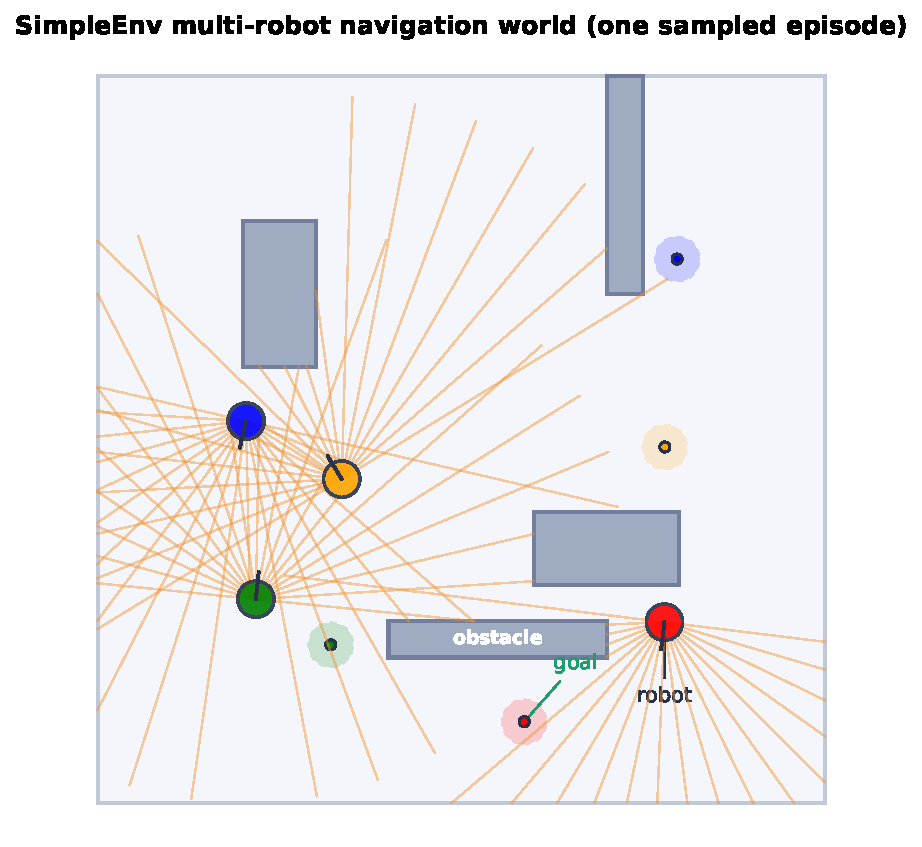
\includegraphics[width=0.8\linewidth]{environment.pdf}
  \caption{The \emph{SimpleEnv} world (one sampled episode, four active
  robots). Each robot (coloured disc with a heading tick) casts a
  $20$-beam lidar fan (orange) that terminates at the nearest obstacle,
  wall or other robot; the matching-coloured dot with a dashed halo is
  that robot's goal and its arrival tolerance.}
  \label{fig:env}
\end{figure}

\begin{figure}[H]
  \centering
  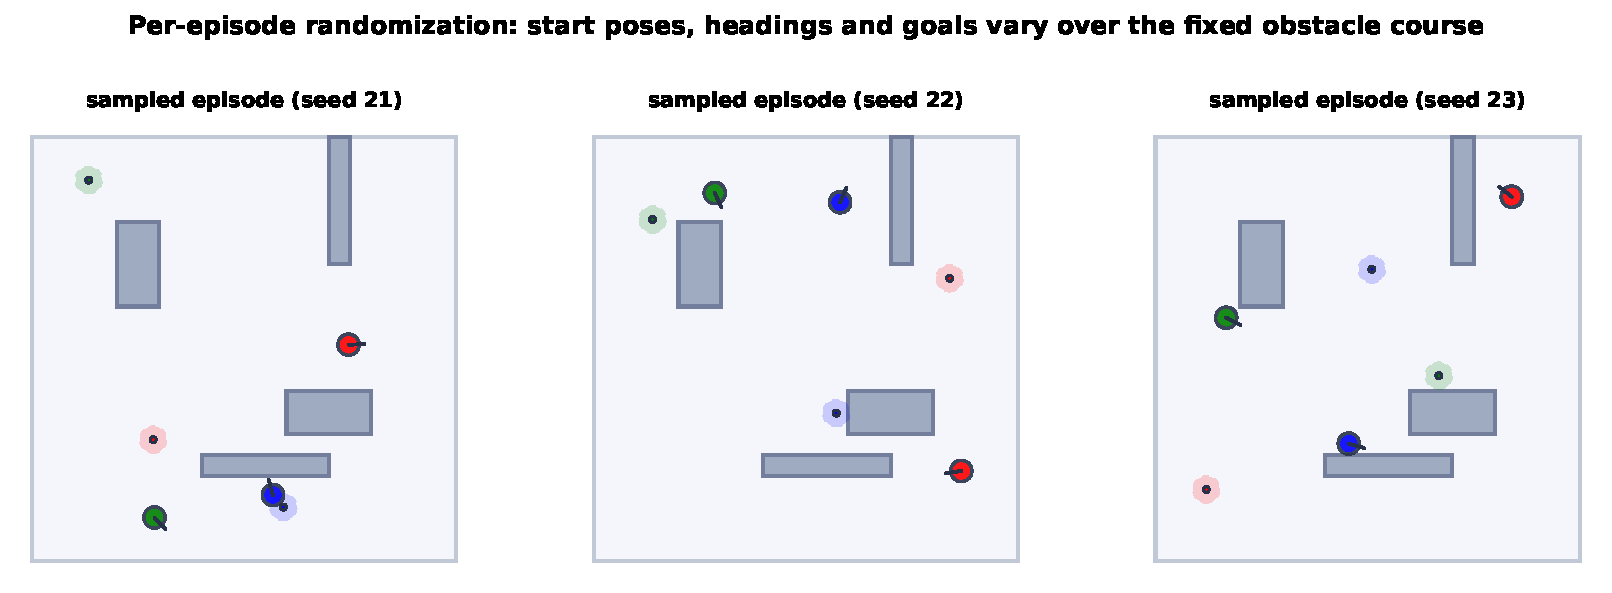
\includegraphics[width=0.98\linewidth]{layouts.pdf}
  \caption{Three independently sampled episodes. The obstacle course is
  fixed; start positions, headings and goals are re-drawn every episode,
  so the policy cannot memorise a single route assignment.}
  \label{fig:layouts}
\end{figure}

\subsection{Markov decision process}
Each robot runs the same policy on its own observation; the per-robot
decision problem is the following MDP.

\paragraph{State $s\in\R^{24}$.}
The observation concatenates the $20$ normalised lidar ranges
$d_1,\dots,d_{20}\in[0,1]$ with four scalars — the normalised distance and
relative bearing to the robot's own goal, and its current velocities:
\begin{equation}
s = \big(\,d_1,\dots,d_{20},\;\tfrac{\rho_g}{L},\;
\tfrac{\Delta\phi}{\pi},\;v,\;\omega\,\big),
\end{equation}
where $\rho_g$ is the Euclidean distance to the goal, $L=\sqrt{10^2+10^2}$
the world diagonal, $\Delta\phi \in [-\pi, \pi)$ the \emph{signed} heading
error toward the goal, and $v,\omega$ the linear and angular velocity applied
at the previous step. Nothing in the state identifies the other robots
explicitly; they enter only through the lidar ranges.

\paragraph{Action $a\in[-1,1]^2$.}
The actor emits $(a_0, a_1)$ through a $\tanh$ output. The entry points remap
the throttle to a forward-only velocity, $v = \tfrac{a_0+1}{2}\in[0,1]$, keep
$\omega = a_1$, and integrate the unicycle model with $\Delta t = 0.1$:
\begin{align}
\theta &\leftarrow \theta + \omega\,\Delta t, &
x &\leftarrow x + v\cos\theta\,\Delta t, &
y &\leftarrow y + v\sin\theta\,\Delta t.
\end{align}

\paragraph{Reward.}
Each robot receives its own reward: large terminal bonuses/penalties plus a
dense step shaping that rewards forward speed and penalises turning,
obstacle proximity and time:
\begin{equation}
r =
\begin{cases}
+100 & \text{goal reached } (\rho_g < 0.3),\\
-100 & \text{collision (obstacle, wall or another robot)},\\
\tfrac{v}{2} - \tfrac{|\omega|}{2}
  - \max(0,\,1 - d_{\min}) - 0.05 & \text{otherwise,}
\end{cases}
\end{equation}
where $d_{\min}$ is the smallest current lidar reading. A robot's episode
ends on arrival, collision, or after $500$ steps; finished robots freeze in
place (remaining lidar-visible to the others) until the episode ends for
everyone.

\section{Method}
\subsection{Twin Delayed DDPG}
DDPG~\cite{lillicrap2016} learns a deterministic actor $\mu_\theta(s)$
alongside a critic $Q_\psi(s,a)$, but its critic systematically overestimates
values and the actor exploits those errors. TD3~\cite{fujimoto2018} adds
three fixes, all present here (Figure~\ref{fig:arch}). \emph{Twin critics}:
two Q heads are trained on the same target, and the target value takes their
minimum. \emph{Target-policy smoothing}: the target action is perturbed with
clipped Gaussian noise, regularising the value estimate over a neighbourhood
of actions:
\begin{align}
\tilde a &= \mu_{\theta'}(s_{t+1})
  + \operatorname{clip}(\epsilon, -c, c),
  \qquad \epsilon \sim \mathcal{N}(0, \sigma^2),\\
y_t &= r_t + \gamma\,(1-\text{done})\,
  \min_{k=1,2} Q_{\psi_k'}\!\big(s_{t+1}, \tilde a\big),
\end{align}
with $\sigma=0.2$, $c=0.5$. \emph{Delayed updates}: both critics are updated
every iteration on the MSE to $y_t$, while the actor and all target networks
(Polyak averaging, $\tau=0.005$) are updated every second iteration only,
letting the value estimate settle before the policy moves. Updates are run at
the end of each episode, one iteration per environment step collected.

\begin{figure}[H]
  \centering
  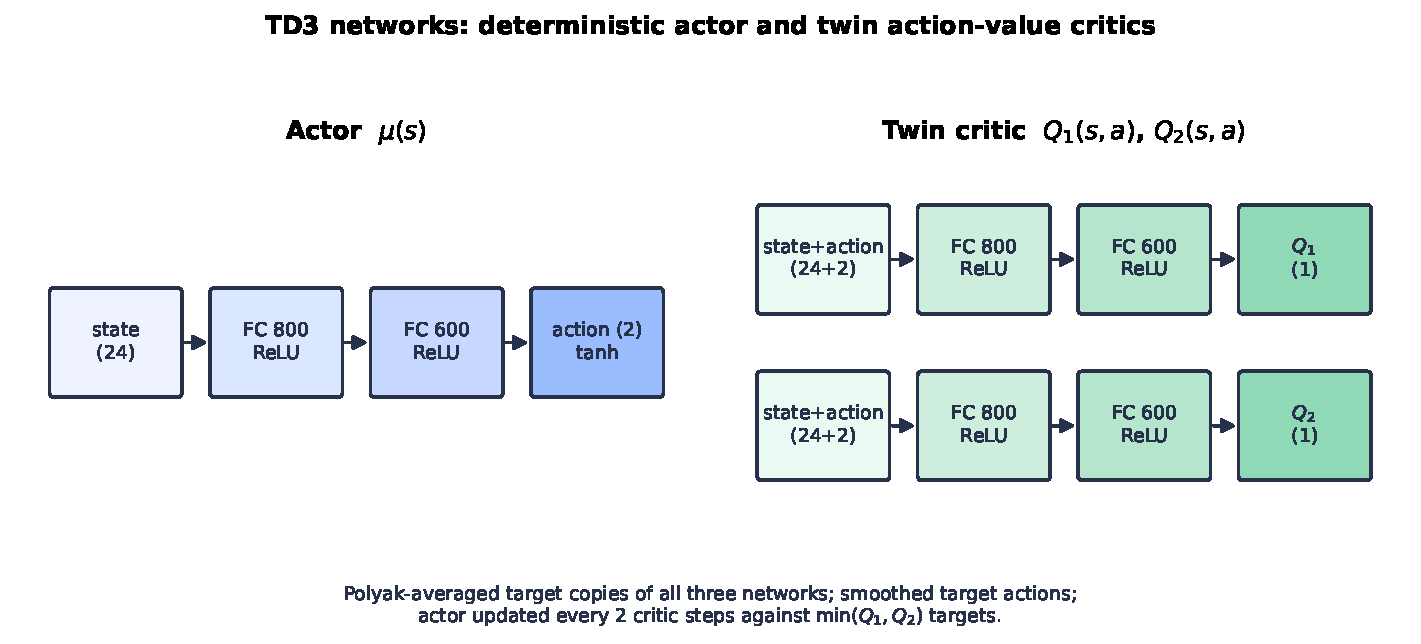
\includegraphics[width=0.98\linewidth]{architecture.pdf}
  \caption{The TD3 networks. The actor maps a $24$-d observation to a $2$-d
  $\tanh$ action; the twin critic scores a state--action pair ($26$ inputs)
  with two independent $Q$ heads whose minimum forms the learning target.}
  \label{fig:arch}
\end{figure}

\paragraph{Exploration.}
Actions are perturbed with Gaussian noise whose scale decays linearly from
$1.0$ to $0.1$ over the first $5\times10^5$ timesteps, then stays at $0.1$;
the sum is clipped to the action bounds.

\subsection{Multi-agent training: parameter sharing and a curriculum}
All robots execute the \emph{same} network. At every environment step the
shared actor is queried once per active robot on that robot's own
observation, and each robot's transition
$(s_i, a_i, r_i, s_i')$ is pushed into one shared replay
buffer~\cite{gupta2017}. With $n$ robots active, every environment step
therefore contributes $n$ transitions, and the critic learns from the
interaction patterns of all robots at once.

From any single robot's perspective the others make the environment
non-stationary~\cite{tan1993}: the same action in the same observed state
can succeed or fail depending on what the rest of the team does next. To
soften this, training follows a \emph{robot-count
curriculum}~\cite{bengio2009}: each episode draws its active robot count
uniformly from $\{1, \dots, n_{\max}(t)\}$, where the cap
$n_{\max}(t) = \min(8, \lfloor 1 + 8t/T_{\mathrm{ramp}} \rfloor)$ grows
stepwise from $1$, reaching \CurriculumCap{} at $7\times10^5$ of the $10^6$
training timesteps ($T_{\mathrm{ramp}} = 8\times10^5$). Early training thus
learns single-robot
navigation on a quiet map; multi-robot interference is introduced only once
the basic competence exists.

\section{Implementation}
The system is implemented in PyTorch as an installable \texttt{src}-layout
package (\texttt{multiagent\_navigation}) with Hydra-based configuration, a
pure-logic training core (\texttt{lib.train}), and thin command-line entry
points. The environment capacity, curriculum cap and schedule are all typed
config fields, so sweeps over team size are one-line Hydra overrides. Device
selection prefers CUDA, then Apple MPS, then CPU, and lives only in the entry
points — the library itself is device-agnostic. Quality is enforced at
commit time (Ruff, strict mypy, property-based tests, custom style checks).
Every $5000$ timesteps the policy is evaluated on $100$ fresh episodes
(deterministic actions, no exploration noise) and checkpointed; the
evaluation log is the data behind Section~\ref{sec:results}.
Table~\ref{tab:hp} lists the hyperparameters.

\begin{table}[H]
  \centering
  \caption{Training hyperparameters (the composed Hydra config).}
  \label{tab:hp}
  \begin{tabular}{llll}
    \toprule
    Parameter & Value & Parameter & Value\\
    \midrule
    Timesteps             & $10^6$          & Replay capacity  & $600{,}000$\\
    Max steps / episode   & $500$           & Batch size       & $256$\\
    Discount $\gamma$     & $0.9999$        & Actor LR (Adam)  & $1\!\times\!10^{-4}$\\
    Soft-update $\tau$    & $0.005$         & Critic LR (Adam) & $5\!\times\!10^{-4}$\\
    Policy delay          & $2$             & Smoothing noise  & $0.2$ (clip $0.5$)\\
    Expl.\ noise          & $1 \to 0.1$     & over             & $5\!\times\!10^5$ steps\\
    Curriculum cap        & \CurriculumCap{} robots & over     & $8\!\times\!10^5$ steps\\
    Hidden units          & $800, 600$      & Eval             & $100$ ep.\ / $5000$ steps\\
    \bottomrule
  \end{tabular}
\end{table}

\section{Experiments and Results}
\label{sec:results}
\paragraph{Setup.}
All numbers in this section are computed from the curated evaluation log of
the training run (\texttt{report/assets/TD3\_simpleEnv.json}, \NumEpochs{}
evaluation epochs). Each epoch reports per-robot averages over $100$
deterministic evaluation episodes; the evaluation robot count follows the
training curriculum, so early epochs measure single-robot navigation and
late epochs the full \CurriculumCap-robot task. An episode outcome is
counted per robot: \emph{arrived}, \emph{collision} or \emph{timeout}.

\paragraph{Learning dynamics.}
Figure~\ref{fig:lc} shows the training curves with the curriculum phases
shaded. The mean per-robot return climbs from \EarlyReturn{} over the first
ten epochs to strongly positive once single-robot navigation is mastered;
the arrival rate reaches \PeakArrived{} (collision rate \PeakCollision) in
epoch~\PeakEpoch{} while \PeakRobots{} robots are active, and the policy
carries this skill into the full \CurriculumCap-robot phase almost intact:
its first ten \CurriculumCap-robot epochs average $89.6\%$ arrivals, peaking
at \BestArrived{} (collision rate \BestCollision) in epoch~\BestEpoch{},
about $7 \times 10^5$ timesteps in. Epoch~\BestEpoch{} is the checkpoint we
publish; re-evaluated on $100$ freshly sampled \CurriculumCap-robot
episodes it delivers \FreshArrived{} arrivals (\FreshCollision{} collisions,
\FreshTimeout{} timeouts).

\paragraph{Late-training degradation.}
Training \emph{past} that point makes the policy worse, not better: over the
final $20$ epochs — all at a fixed $n = \CurriculumCap$ — arrivals average
only \LateArrived{} while collisions average \LateCollision{}, and the last
epochs fall below $60\%$. Two observations localise the cause. First,
timeouts stay near zero throughout (\LateTimeout{} late-window mean): the
swarm never loses the ability to reach goals, it loses caution — failures
convert almost one-for-one into collisions. Second, the slide starts only
after ${\sim}7.8 \times 10^5$ timesteps, by which point the
$6 \times 10^5$-transition replay buffer (multiple transitions per
timestep with many robots) has fully turned over to recent, high-skill
experience: the critic no longer sees what risky manoeuvres cost, while the
$+v/2$ speed term keeps rewarding faster driving, pushing the co-adapting
robots into an aggressive, collision-prone regime. Per-epoch checkpointing
plus selection on the evaluation log — early stopping — is the remedy this
pipeline builds in; larger buffers, a lower discount or a decaying learning
rate are the natural mitigations left to future work.

\begin{figure}[H]
  \centering
  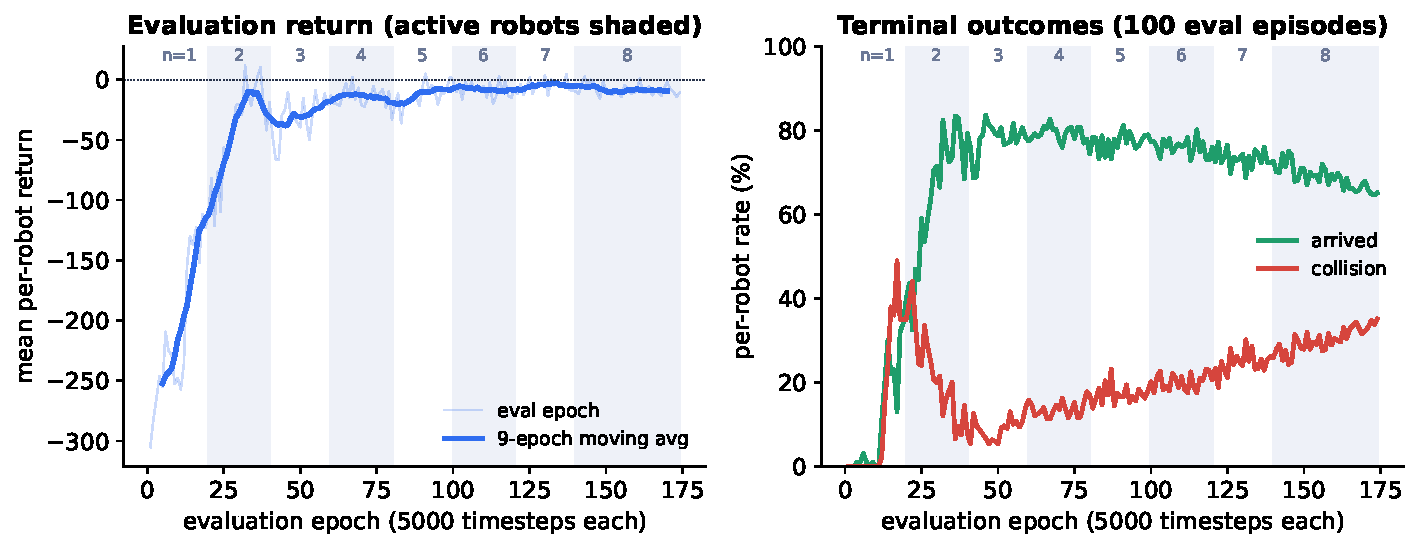
\includegraphics[width=0.98\linewidth]{learning_curve.pdf}
  \caption{Left: mean per-robot evaluation return (faint) with a $9$-epoch
  moving average. Right: per-robot arrival and collision rates. Shaded bands
  mark the curriculum phases; the label is the active robot count $n$
  during evaluation.}
  \label{fig:lc}
\end{figure}

\paragraph{Interference, not incompetence.}
At its selected checkpoint the policy loses only a few points when the world
fills up: \PeakArrived{} of robots arrive at $n=\PeakRobots$ versus
\BestArrived{} at $n=\CurriculumCap$, with the gap absorbed almost entirely
by the collision rate (\PeakCollision{} $\to$ \BestCollision). Since
finished robots freeze in place and remain lidar-visible, late-episode
worlds are also more cluttered than the obstacle course alone. Both the
residual gap and the late-training collapse point the same way: coordination
— not single-robot skill — is the binding constraint, and parameter sharing
alone does not resolve it: the robots share competence but not intent.

\begin{figure}[H]
  \centering
  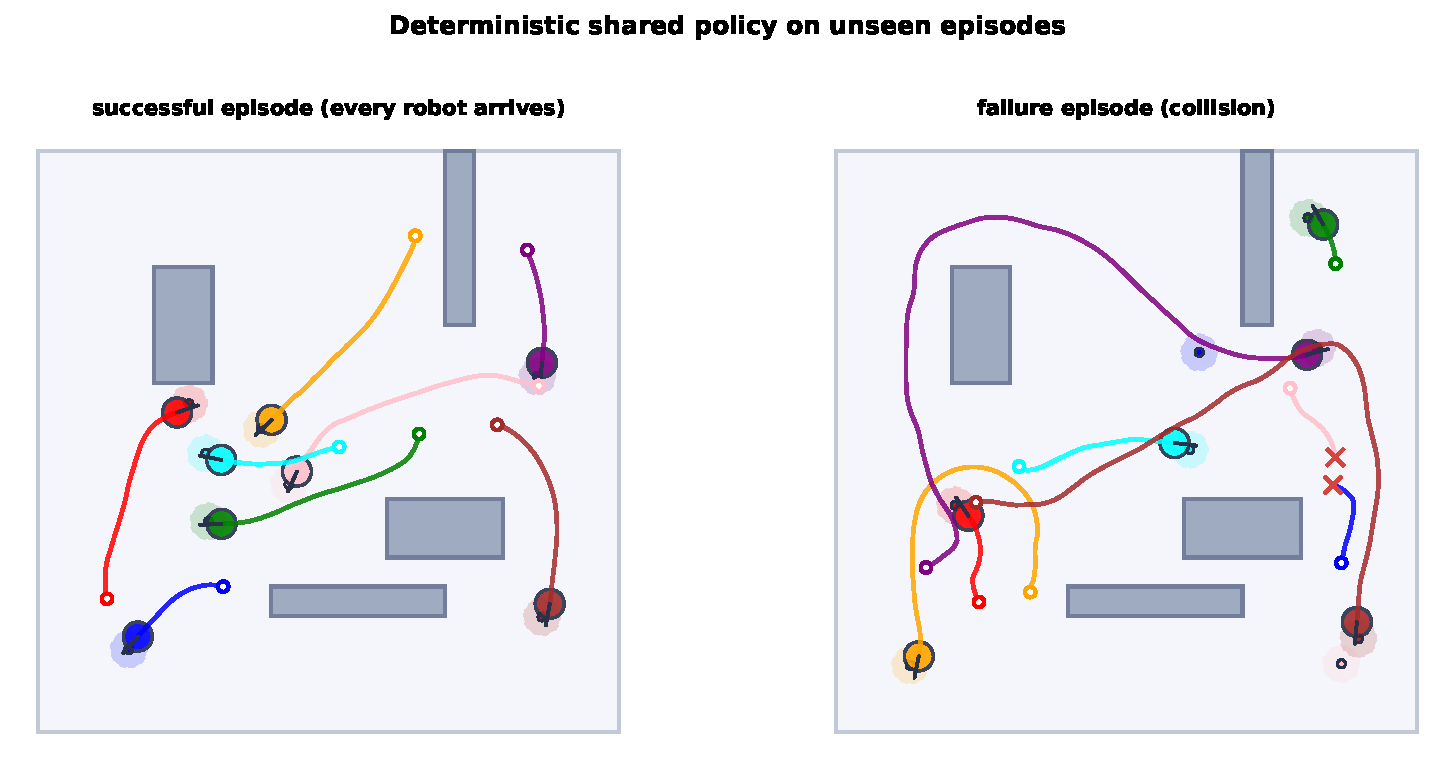
\includegraphics[width=0.98\linewidth]{trajectory.pdf}
  \caption{The deterministic shared policy on unseen episodes. Left: every
  robot reaches its goal. Right: a characteristic failure — paths cross
  and a robot collides.}
  \label{fig:traj}
\end{figure}

\section{Visualisation}
The package ships a vector renderer (\texttt{viz.py}) with two faces. A
live \texttt{FuncAnimation} viewer replays the best checkpointed epoch and
dumps every robot's $24$-d observation per step to a CSV for offline
analysis. The same module's drawing helpers (field, obstacles, per-robot
goals, lidar fans, trajectories) back every figure in this report, and the
repository ships a script that renders policy rollouts into an animated GIF
for the README, so the paper and the live environment are guaranteed to
agree. All figures are emitted as scalable PDF.

\section{Conclusion and Future Work}
We presented a complete multi-robot navigation agent: a single TD3 policy,
trained with parameter sharing on the pooled experience of a growing robot
team, that navigates lidar-only robots to individual goals among obstacles.
On real training data the shared policy masters navigation early
(\PeakArrived{} arrivals at \PeakRobots{} robots) and, selected by early
stopping, retains \BestArrived{} per-robot arrivals at the full
\CurriculumCap-robot task (\FreshArrived{} on fresh episodes), with
robot--robot collisions as the dominant remaining failure mode — both in
the residual gap and in the late-training degradation that continued
optimisation induces. Natural next steps target exactly these gaps:
centralized critics with decentralized actors, inter-robot communication or
attention over neighbouring robots, explicit collision-avoidance shaping
between robots, larger or prioritised replay against the late-stage buffer
turnover, and randomising the obstacle course itself for cross-layout
generalization.

\begin{thebibliography}{9}
\bibitem{fujimoto2018} S.~Fujimoto, H.~van Hoof, and D.~Meger,
``Addressing function approximation error in actor-critic methods,'' in
\emph{ICML}, 2018.
\bibitem{lillicrap2016} T.~P.~Lillicrap, J.~J.~Hunt, A.~Pritzel, et~al.,
``Continuous control with deep reinforcement learning,'' in \emph{ICLR}, 2016.
\bibitem{silver2014} D.~Silver, G.~Lever, N.~Heess, et~al.,
``Deterministic policy gradient algorithms,'' in \emph{ICML}, 2014.
\bibitem{mnih2015} V.~Mnih, K.~Kavukcuoglu, D.~Silver, et~al.,
``Human-level control through deep reinforcement learning,''
\emph{Nature}, vol.~518, pp.~529--533, 2015.
\bibitem{sutton2018} R.~S.~Sutton and A.~G.~Barto,
\emph{Reinforcement Learning: An Introduction}, 2nd ed. MIT Press, 2018.
\bibitem{tan1993} M.~Tan,
``Multi-agent reinforcement learning: independent vs.\ cooperative agents,''
in \emph{ICML}, 1993.
\bibitem{gupta2017} J.~K.~Gupta, M.~Egorov, and M.~Kochenderfer,
``Cooperative multi-agent control using deep reinforcement learning,'' in
\emph{AAMAS Workshops}, 2017.
\bibitem{long2018} P.~Long, T.~Fan, X.~Liao, et~al.,
``Towards optimally decentralized multi-robot collision avoidance via deep
reinforcement learning,'' in \emph{ICRA}, 2018.
\bibitem{bengio2009} Y.~Bengio, J.~Louradour, R.~Collobert, and J.~Weston,
``Curriculum learning,'' in \emph{ICML}, 2009.
\end{thebibliography}

\end{document}
